\chapter{Entwurf} \label{chap:entwurf}

\section{Architektur der Datenbank} \label{sec:DB}
\begin{figure}[ht]
    \centering
    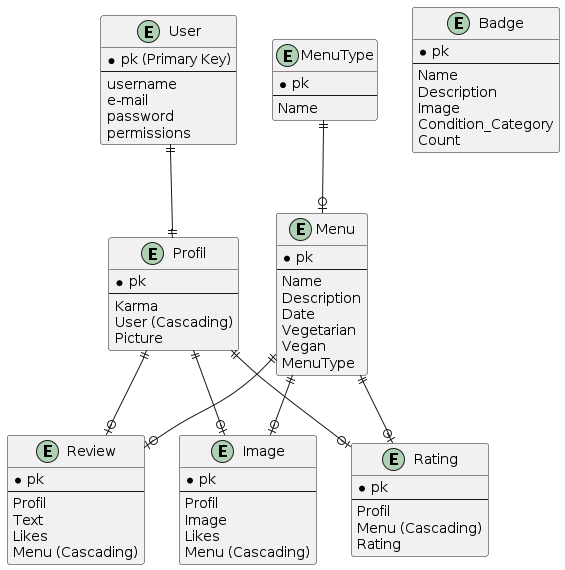
\includegraphics[width=0.8\textwidth]{images/Database.png}
    \caption{Architektur der Datenbank siehe auch \ref{code:core.models.py}}
    \label{fig:DB}
\end{figure}

Diese Skizze repräsentiert den Aufbau der Datenbank. Sie zeigt die verschiedenen
Entities und ihre Relationships. Die Datenbankstruktur ist in der Datei
\code{core/models.py} beschrieben (siehe \ref{code:core.models.py}).

\section{UML-Diagramm der WebApp} \label{sec:UMLS}
\begin{figure}[ht]
    \centering
    
\includegraphics[width=0.4\textwidth]{images/UML-Specific.png}
    \caption{UML Diagramm der WebApp}
    \label{fig:DB}
\end{figure}

Dieses UML-Diagramm zeigt die Zusammenhänge aller Komponenten (nicht Klassen,
häufig einfach Funktionen) der WebApp. Dabei sind nur die Verbindungen der
\code{Index} Seite und der \code{Menu} Seite vorhanden, da es mit allen
Verbindungen zu unübersichtlich werden würde. Die Rechtecke beschreiben eigene
files, die Quadrate eigene Funktionen und die Pfeile (Verbindungen) beschreiben
Aufrufe von Funktionen in anderen Funktionen.
 
\newpage

\section{Vereinfachtes UML-Diagramm der WebApp} \label{sec:UMLG}
\begin{figure}[ht]
    \centering
    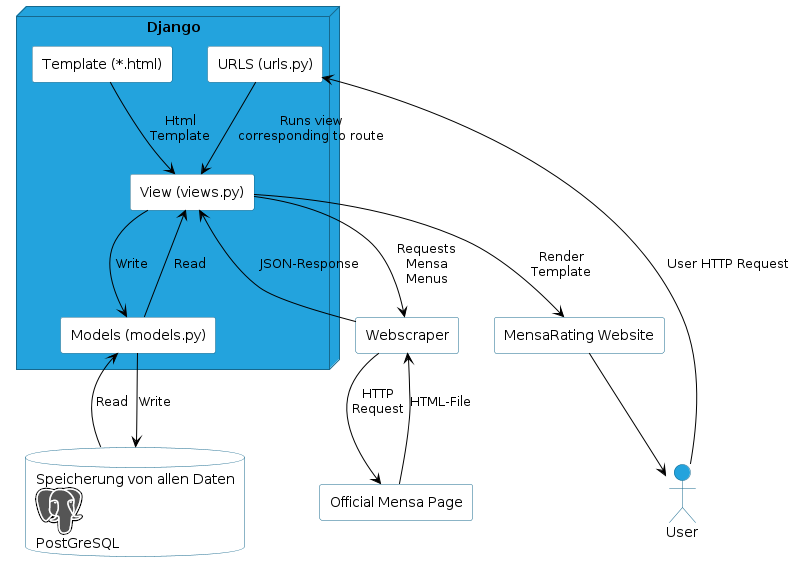
\includegraphics[width=0.8\textwidth]{images/UML-General.png}
    \caption{UML Diagramm (vereinfacht) der WebApp}
    \label{fig:DB}
\end{figure}

Dieses UML-Diagramm ist weniger spezifisch als das letzte (siehe
\ref{sec:UMLS}). Im Gegensatz zum letzten Diagramm zeigt dieses allerdings alle
wichtigen Verbindungen der einzelnen Komponenten der WebApp (Django, die
Datenbank, die Webseite, die offizielle Mensa Webseite und der User)


